% Eine Quelle, zwei PDFs. scripts/build.sh setzt \explainmode:
%   0 -> loesung_blatt02.pdf
%   1 -> erklaerung_blatt02.pdf
\documentclass[a4paper,11pt]{article}
\usepackage[T1]{fontenc}
\usepackage[utf8]{inputenc}
\usepackage[english]{babel}
\usepackage{amsmath,amssymb,mathtools}
\usepackage[margin=2.2cm]{geometry}
\usepackage{enumitem}
\usepackage{xcolor}
\usepackage{booktabs}
\usepackage{tikz}
\usetikzlibrary{patterns,arrows.meta}
\usepackage{pgfplots}\pgfplotsset{compat=1.18}
\usepackage[most]{tcolorbox}
\setlength{\parindent}{0pt}
\setlength{\parskip}{4pt}

\providecommand{\explainmode}{0}
\newif\ifexplain
\ifnum\explainmode=1 \explaintrue\fi

\newcommand{\blatttitel}[2]{\begin{center}{\Large\bfseries #1}\\[2pt]#2\end{center}}
\newcommand{\aufgabe}[1]{\section*{#1}}
\newcommand{\angabe}[1]{\textit{#1}\par\smallskip}
\newcommand{\teil}[1]{\subsection*{(#1)}}
\newcommand{\why}[1]{\text{\small\color{black!65}#1}}

\newtcolorbox{erklbox}{colback=blue!4,colframe=blue!40,breakable,boxrule=0.5pt,
  fonttitle=\bfseries\small,title={Erklärung}}
\newcommand{\explain}[1]{\ifexplain\begin{erklbox}#1\end{erklbox}\fi}
\newcommand{\explainfig}[1]{\ifexplain\begin{center}#1\end{center}\fi}

\begin{document}
\blatttitel{Exercise sheet 2 -- \ifexplain Explanation\else Solution\fi}{Linear Optimization (WS 26/27)}

\explain{Dieses Blatt behandelt drei Grundideen: Gleichungssysteme mit mehr Variablen als Gleichungen, die Standardform aus der Vorlesung und graphisches Lösen linearer Programme. Bei der Standardform im Skript wird ein Maximierungsproblem mit Gleichungen $Ax=b$ und Nichtnegativität $x\ge0$ verwendet.}

\aufgabe{Classroom task 2.1}
\angabe{What happens to the solution $(x_1,x_2)$ of the linear system $Ax=b$ with $A=\begin{pmatrix}1&1\\0&3\end{pmatrix}$ and $b=\begin{pmatrix}2\\3\end{pmatrix}$ if we add a column to the matrix on the left hand side, so that $\widetilde A=\begin{pmatrix}1&1&0\\0&3&1\end{pmatrix}$? How can we represent the solution to the new system?}
\explain{Zuerst lösen wir das alte System. Danach bekommt das neue System eine zusätzliche Variable $x_3$. Weil dann zwei Gleichungen und drei Variablen vorhanden sind, wird eine Variable als freier Parameter gewählt.}

The original system is
\[
\begin{pmatrix}1&1\\0&3\end{pmatrix}
\begin{pmatrix}x_1\\x_2\end{pmatrix}
=
\begin{pmatrix}2\\3\end{pmatrix}.
\]
It is equivalent to
\begin{align*}
x_1+x_2&=2 && \why{row $1$ of $Ax=b$}\\
3x_2&=3 && \why{row $2$ of $Ax=b$}
\end{align*}
Solving the second equation gives
\begin{align*}
3x_2&=3 && \why{second equation}\\
x_2&=1 && \why{$|\,/3$}
\end{align*}
Substitute this value into the first equation:
\begin{align*}
x_1+x_2&=2 && \why{first equation}\\
x_1+1&=2 && \why{insert $x_2=1$}\\
x_1&=1 && \why{$|\,-1$}
\end{align*}
\explain{Das alte System hat genau eine Lösung, weil die beiden Gleichungen zwei Variablen festlegen.}
Thus the original solution is
\[
\begin{pmatrix}x_1\\x_2\end{pmatrix}
=
\begin{pmatrix}1\\1\end{pmatrix}.
\]

The new system is
\[
\begin{pmatrix}1&1&0\\0&3&1\end{pmatrix}
\begin{pmatrix}x_1\\x_2\\x_3\end{pmatrix}
=
\begin{pmatrix}2\\3\end{pmatrix}.
\]
It is equivalent to
\begin{align*}
x_1+x_2&=2 && \why{row $1$ of $\widetilde Ax=b$}\\
3x_2+x_3&=3 && \why{row $2$ of $\widetilde Ax=b$}
\end{align*}
Let
\begin{align*}
x_3&=t && \why{choose the new variable as a parameter}
\end{align*}
Then the second equation gives
\begin{align*}
3x_2+x_3&=3 && \why{second equation}\\
3x_2+t&=3 && \why{insert $x_3=t$}\\
3x_2&=3-t && \why{$|\,-t$}\\
x_2&=1-\frac{t}{3} && \why{$|\,/3$}
\end{align*}
Now the first equation gives
\begin{align*}
x_1+x_2&=2 && \why{first equation}\\
x_1+1-\frac{t}{3}&=2 && \why{insert $x_2=1-\frac{t}{3}$}\\
x_1-\frac{t}{3}&=1 && \why{$|\,-1$}\\
x_1&=1+\frac{t}{3} && \why{$|\,+\frac{t}{3}$}
\end{align*}
\explain{Der Parameter $t$ kann jede reelle Zahl sein. Daher ist die neue Lösungsmenge eine Gerade im dreidimensionalen Raum.}
Check:
\begin{align*}
x_1+x_2&=1+\frac{t}{3}+1-\frac{t}{3} && \why{insert $x_1$ and $x_2$}\\
&=2 && \why{$\frac{t}{3}-\frac{t}{3}=0$}\\
3x_2+x_3&=3\left(1-\frac{t}{3}\right)+t && \why{insert $x_2$ and $x_3$}\\
&=3-t+t && \why{distribute $3$}\\
&=3 && \why{$-t+t=0$}
\end{align*}
\[
\boxed{\left\{\begin{pmatrix}1+\frac{t}{3}\\[1mm]1-\frac{t}{3}\\[1mm]t\end{pmatrix}\,\middle|\,t\in\mathbb R\right\}}
\]

\aufgabe{Exercise 2.1}
\angabe{Consider the linear optimization problem $\max\{2x_1+x_2\mid 2x_1-x_2\le 12,\ 0\le x_1\le 8,\ x_2\ge0\}$. Transform the problem into standard form and explicitly define $c$, $b$ and $A$ as in the lecture notes. Is the problem feasible? Is the problem bounded?}
\explain{Die Vorlesungs-Standardform lautet: maximize $c^Tx$ subject to $Ax=b$ and $x\ge0$. Deshalb werden die Ungleichungen mit Schlupfvariablen in Gleichungen umgeschrieben.}

The lecture standard form is
\[
\begin{array}{ll}
\text{maximize} & c^Tx\\
\text{subject to} & Ax=b,\\
& x\ge0.
\end{array}
\]
The constraint $0\le x_1\le8$ gives nonnegativity of $x_1$ and the upper bound
\begin{align*}
x_1&\le 8 && \why{upper bound from $0\le x_1\le8$}
\end{align*}
Introduce slack variables $s_1,s_2\ge0$:
\begin{align*}
2x_1-x_2+s_1&=12 && \why{add slack variable $s_1$ to the first inequality}\\
x_1+s_2&=8 && \why{add slack variable $s_2$ to the upper bound}
\end{align*}
Define
\[
y=(x_1,x_2,s_1,s_2)^T.
\]
Then
\[
A=\begin{pmatrix}
2&-1&1&0\\
1&0&0&1
\end{pmatrix},\qquad
b=\begin{pmatrix}12\\8\end{pmatrix},\qquad
c=\begin{pmatrix}2\\1\\0\\0\end{pmatrix}.
\]
\explain{Die Nullen in $c$ stehen dort, weil die Schlupfvariablen nur Nebenbedingungen ausgleichen und nicht in der ursprünglichen Zielfunktion vorkommen.}
The standard form is
\[
\boxed{
\begin{array}{ll}
\text{maximize} & 2x_1+x_2\\[1mm]
\text{subject to} & 2x_1-x_2+s_1=12,\\
& x_1+s_2=8,\\
& x_1,x_2,s_1,s_2\ge0.
\end{array}}
\]

Feasibility check:
Choose
\[
y=(0,0,12,8)^T.
\]
\begin{align*}
2\cdot0-0+12+0&=12 && \why{first row of $Ay$}\\
0+8&=8 && \why{second row of $Ay$}
\end{align*}
Thus $Ay=b$.
Also
\begin{align*}
y&\ge0 && \why{all entries $0,0,12,8$ are nonnegative}
\end{align*}
Therefore the problem is feasible.

Boundedness check:
For every $M\ge0$, choose
\[
y(M)=(0,M,12+M,8)^T.
\]
Then
\begin{align*}
2\cdot0-M+12+M&=12 && \why{first row of $Ay(M)$}\\
0+8&=8 && \why{second row of $Ay(M)$}
\end{align*}
Thus $Ay(M)=b$.
The objective value is
\begin{align*}
c^Ty(M)&=2\cdot0+M+0\cdot(12+M)+0\cdot8 && \why{insert $y(M)$}\\
&=M && \why{terms with factor $0$ vanish}
\end{align*}
\explain{Da $M$ beliebig groß gewählt werden kann, werden auch die Zielfunktionswerte beliebig groß. Das ist bei Maximierung genau Unbeschränktheit.}
\[
\boxed{\text{The problem is feasible and unbounded.}}
\]

\aufgabe{Exercise 2.2}
\angabe{Determine the linear program that was solved graphically in Figure 1. Standard form is not required. The figure shows a feasible region to the right of $x_1=3$, above the line through $(0,4)$ and $(6,0)$, and above the line through $(1,0)$ and $(7,3)$. The red objective lines have slope $-2$ and touch the feasible region first at $(3,2)$.}
\explain{Aus einer gezeichneten Geraden lesen wir zwei Punkte ab. Daraus wird ihre Gleichung bestimmt. Bei einer Zielfunktionsgeraden $c_1x_1+c_2x_2=\alpha$ ist die Steigung $-c_1/c_2$. Die rote Steigung $-2$ passt zu $2x_1+x_2=\alpha$.}

The vertical boundary gives
\begin{align*}
x_1&\ge3 && \why{feasible region is to the right of the line $x_1=3$}
\end{align*}
The blue boundary passes through $(0,4)$ and $(6,0)$. Its slope is
\begin{align*}
m&=\frac{0-4}{6-0} && \why{slope formula}\\
&=-\frac{4}{6} && \why{compute numerator and denominator}\\
&=-\frac{2}{3} && \why{divide numerator and denominator by $2$}
\end{align*}
Thus the blue line has equation
\begin{align*}
x_2&=4-\frac{2}{3}x_1 && \why{intercept $4$ and slope $-\frac23$}\\
3x_2&=12-2x_1 && \why{$|\,\cdot3$}\\
2x_1+3x_2&=12 && \why{$|\,+2x_1$}
\end{align*}
The feasible region is above that line, hence
\begin{align*}
2x_1+3x_2&\ge12 && \why{choose the side above the blue line}
\end{align*}
The rising boundary passes through $(1,0)$ and $(7,3)$. Its slope is
\begin{align*}
m&=\frac{3-0}{7-1} && \why{slope formula}\\
&=\frac{3}{6} && \why{compute numerator and denominator}\\
&=\frac{1}{2} && \why{divide numerator and denominator by $3$}
\end{align*}
Using the point $(1,0)$ gives
\begin{align*}
x_2-0&=\frac12(x_1-1) && \why{point-slope form}\\
x_2&=\frac12x_1-\frac12 && \why{distribute $\frac12$}\\
2x_2&=x_1-1 && \why{$|\,\cdot2$}\\
-x_1+2x_2&=-1 && \why{$|\,-x_1$}
\end{align*}
The feasible region is above that line, hence
\begin{align*}
-x_1+2x_2&\ge-1 && \why{choose the side above the rising line}
\end{align*}
The red objective lines have slope $-2$, so one matching objective is
\begin{align*}
z&=2x_1+x_2 && \why{line $2x_1+x_2=\alpha$ has slope $-2$}
\end{align*}
Because the shaded region is unbounded to the upper right, the graph solves a minimization problem. Therefore one equivalent linear program represented by the figure is
\[
\boxed{
\begin{array}{ll}
\text{minimize} & 2x_1+x_2\\[1mm]
\text{subject to} & x_1\ge3,\\
& 2x_1+3x_2\ge12,\\
& -x_1+2x_2\ge-1.
\end{array}}
\]
Check the marked point:
\begin{align*}
2\cdot3+3\cdot2&=6+6 && \why{insert $(3,2)$ into $2x_1+3x_2$}\\
&=12 && \why{$6+6=12$}\\
3&\ge3 && \why{vertical constraint}\\
-3+2\cdot2&=-3+4 && \why{insert $(3,2)$ into $-x_1+2x_2$}\\
&=1 && \why{$-3+4=1$}\\
1&\ge-1 && \why{compare}
\end{align*}
The objective value at $(3,2)$ is
\begin{align*}
z&=2\cdot3+2 && \why{insert $(3,2)$}\\
&=6+2 && \why{$2\cdot3=6$}\\
&=8 && \why{$6+2=8$}
\end{align*}
\[
\boxed{\text{The graphical optimum is }x^*=(3,2)\text{ with value }8.}
\]

\aufgabe{Exercise 2.3}
\angabe{Solve the following linear program graphically: maximize $3x_1+5x_2$ subject to $x_1+2x_2\le12$, $3x_1+x_2\le16$, $0\le x_2\le4$, and $x_1\ge0$.}
\explain{Beim graphischen Lösen reichen die Eckpunkte der zulässigen Menge: Bei einem linearen Programm nimmt eine lineare Zielfunktion ihr Optimum, falls es existiert, an einem Eckpunkt an. Wir bestimmen die Eckpunkte und vergleichen dort die Zielfunktionswerte.}

The boundary lines are
\begin{align*}
x_1+2x_2&=12 && \why{first inequality as equality}\\
3x_1+x_2&=16 && \why{second inequality as equality}\\
x_2&=0 && \why{lower bound for $x_2$}\\
x_2&=4 && \why{upper bound for $x_2$}\\
x_1&=0 && \why{lower bound for $x_1$}
\end{align*}
Find the intersection of the two slanted boundary lines:
\begin{align*}
x_1+2x_2&=12 && \why{first boundary}\\
3x_1+x_2&=16 && \why{second boundary}
\end{align*}
From the first boundary,
\begin{align*}
x_1+2x_2&=12 && \why{first boundary}\\
x_1&=12-2x_2 && \why{$|\,-2x_2$}
\end{align*}
Insert this into the second boundary:
\begin{align*}
3x_1+x_2&=16 && \why{second boundary}\\
3(12-2x_2)+x_2&=16 && \why{insert $x_1=12-2x_2$}\\
36-6x_2+x_2&=16 && \why{distribute $3$}\\
36-5x_2&=16 && \why{$-6x_2+x_2=-5x_2$}\\
-5x_2&=-20 && \why{$|\,-36$}\\
x_2&=4 && \why{$|\,/(-5)$}
\end{align*}
Then
\begin{align*}
x_1&=12-2x_2 && \why{formula from first boundary}\\
x_1&=12-2\cdot4 && \why{insert $x_2=4$}\\
x_1&=12-8 && \why{$2\cdot4=8$}\\
x_1&=4 && \why{$12-8=4$}
\end{align*}
So one vertex is $(4,4)$.

The vertex on $x_2=0$ and $3x_1+x_2=16$ is found by
\begin{align*}
3x_1+x_2&=16 && \why{second boundary}\\
3x_1+0&=16 && \why{insert $x_2=0$}\\
3x_1&=16 && \why{$3x_1+0=3x_1$}\\
x_1&=\frac{16}{3} && \why{$|\,/3$}
\end{align*}
Thus this vertex is $\left(\frac{16}{3},0\right)$.

The remaining axis vertices are
\begin{align*}
(0,0)&\text{ is feasible} && \why{both lower bounds active}\\
(0,4)&\text{ is feasible} && \why{$x_1=0$ and upper bound $x_2=4$ active}
\end{align*}
\explain{Der Punkt $(0,6)$ aus $x_1+2x_2=12$ ist nicht zulässig, weil $x_2\le4$ gilt. Daher liegt der obere linke Eckpunkt bei $(0,4)$.}

% grafik-verlangt
\begin{center}
% grafik-verlangt
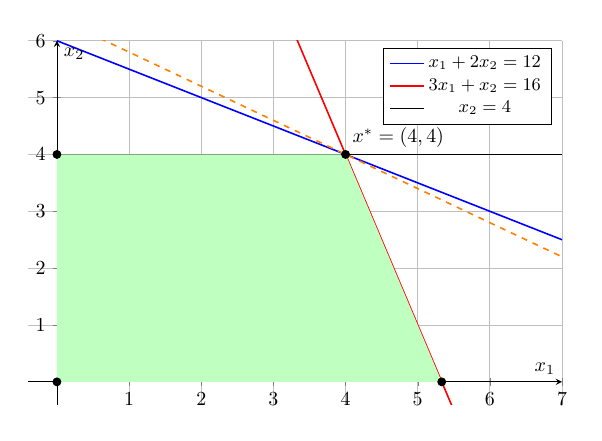
\begin{tikzpicture}[scale=0.72]
  \begin{axis}[
    axis lines=middle,
    xmin=-0.4,xmax=7,
    ymin=-0.4,ymax=6,
    xlabel={$x_1$},ylabel={$x_2$},
    grid=both,
    width=11cm,height=8cm,
    legend style={at={(0.98,0.98)},anchor=north east,font=\small}
  ]
    \addplot[domain=0:7,blue,thick] {(12-x)/2};
    \addlegendentry{$x_1+2x_2=12$}
    \addplot[domain=0:7,red,thick] {16-3*x};
    \addlegendentry{$3x_1+x_2=16$}
    \addplot[black,thick,domain=0:7] {4};
    \addlegendentry{$x_2=4$}
    \addplot[draw=none,fill=green!25] coordinates {(0,0) (5.333,0) (4,4) (0,4)} -- cycle;
    \addplot[only marks,mark=*,mark size=2pt] coordinates {(0,0) (5.333,0) (4,4) (0,4)};
    \addplot[orange,thick,dashed,domain=0:7] {(32-3*x)/5};
    \node[anchor=south west] at (axis cs:4,4) {$x^*=(4,4)$};
  \end{axis}
\end{tikzpicture}
\end{center}

Evaluate the objective function $z=3x_1+5x_2$ at the feasible vertices:
\begin{align*}
z(0,0)&=3\cdot0+5\cdot0 && \why{insert $(0,0)$}\\
&=0 && \why{compute}\\
z\left(\frac{16}{3},0\right)&=3\cdot\frac{16}{3}+5\cdot0 && \why{insert $\left(\frac{16}{3},0\right)$}\\
&=16+0 && \why{$3\cdot\frac{16}{3}=16$}\\
&=16 && \why{$16+0=16$}\\
z(4,4)&=3\cdot4+5\cdot4 && \why{insert $(4,4)$}\\
&=12+20 && \why{$3\cdot4=12$ and $5\cdot4=20$}\\
&=32 && \why{$12+20=32$}\\
z(0,4)&=3\cdot0+5\cdot4 && \why{insert $(0,4)$}\\
&=0+20 && \why{$3\cdot0=0$ and $5\cdot4=20$}\\
&=20 && \why{$0+20=20$}
\end{align*}
\explain{Der größte Wert in der Liste ist $32$. Die gestrichelte orange Zielfunktionsgerade im Bild ist $3x_1+5x_2=32$ und berührt die zulässige Menge im Punkt $(4,4)$.}
Check feasibility of the optimal point:
\begin{align*}
4+2\cdot4&=4+8 && \why{insert $(4,4)$ into $x_1+2x_2$}\\
&=12 && \why{$4+8=12$}\\
12&\le12 && \why{first constraint is satisfied}\\
3\cdot4+4&=12+4 && \why{insert $(4,4)$ into $3x_1+x_2$}\\
&=16 && \why{$12+4=16$}\\
16&\le16 && \why{second constraint is satisfied}\\
0&\le4 && \why{lower bound for $x_2$}\\
4&\le4 && \why{upper bound for $x_2$}\\
4&\ge0 && \why{lower bound for $x_1$}
\end{align*}
\[
\boxed{x^*=(4,4),\qquad z^*=32}
\]

\end{document}
